\documentclass[a4paper]{article}

% --- LANGUAGE ---

\usepackage[german]{babel}	% language specific quotation marks etc.

% --- DATA ---

\def\lecture{Repetitorium zu Differenzialgleichungen}
\def\authors{Linus Mußmächer}
\def\sheetNumber{03}
\def\sumPoints{30} 

% --- PREAMBLE ---
% === USAGE ===

% when using this preamble, setup your environment variables like this beforehand:


% \title{Stochastik 2}  %Title of exercise 
% \def\lecture{Stochastik 2}
% \def\authors{Linus Mußmächer}
% \def\sheetNumber{02}
% \def\sumPoints{30}      % maximum number of points (leave undefined)

% then use one of these commands (german or english) to print the header:

% \makeexheaderger

% and finally use subsections for your subtasks - they will be numbered as <sheetNumber><task number> by themselves

% if you have an exercise as an external .pdf, use \includetask to include it and increase the task counter


% --- OTHER ---

\usepackage{booktabs}       % professional-quality tables
\usepackage[table]{xcolor}	% color
\usepackage{pdfpages}		% to include entire pdf pages in appendix etc.
\usepackage{enumitem}		% better custom enumerations
\setlist[enumerate, 1]{label=(\roman*)}
\usepackage{etoolbox}		% toolbox for command modification

% --- FONTS & TYPESETTING ---

\usepackage[utf8]{inputenc} % allow utf-8 input
\usepackage[T1]{fontenc}    % use 8-bit T1 fonts
\usepackage{dsfont}			% font with double lines for sets
\usepackage[german,ruled,vlined,linesnumbered,commentsnumbered,algoruled]
{algorithm2e} 				%pseudo code
\usepackage{listings}		%java code
\usepackage{csquotes}

% --- URLS ---

\usepackage[colorlinks=true, linkcolor=black, citecolor=blue, urlcolor=blue]{hyperref}   	% hyperlinks
\usepackage{url}            % simple URL typesetting

% --- MATH SYMBOLS ---

\usepackage{amsmath,amssymb}% more math symbols
\usepackage{amsfonts}       % blackboard math symbols
\usepackage{latexsym}		% more math symbols
\usepackage{chngcntr}		% more math symbols
\usepackage{mathrsfs}		% math-fonts
\usepackage{mathtools}		% more math symbols
\usepackage{nchairx}		% Waldmann package for general math symbols

% --- GRAPHICS & CAPTIONS ----

\usepackage{graphicx}		% including images
\graphicspath{ {./figs/} }
\usepackage{subcaption}		% custom caption formatting
\DeclareCaptionLabelFormat{custom}{ \textbf{#1 #2}}
\captionsetup{format=hang}
\captionsetup{width=0.9\textwidth,labelformat=custom}
\usepackage{pdfpages}		% to include entire pdf pages in appendix etc.

% --- FORMAT ---

\usepackage[a4paper]{geometry} % a4 paper
\usepackage{setspace}		% spacing
\usepackage{titlesec}
\allowdisplaybreaks			% allow page breaks within math environments

% --- CUSTOM COMMANDS ---
%Logic
\newcommand{\then}{\Rightarrow}
\newcommand{\since}{\Leftarrow}
\renewcommand{\iff}{\ensuremath{\Leftrightarrow}}

%pretty epsilon
\let\oldepsilon\epsilon
\let\epsilon\varepsilon
\let\varepsilon\oldepsilon
%pretty phi
\let\oldphi\phi
\let\phi\varphi
\let\varphi\oldphi

\newcommand{\includetask}[2][pages=-]{
    \includepdf[#1]{#2}
    \addtocounter{subsection}{1}
}

% set-up for exercise specific stuff
\ifdef{\sheetNumber}{
    \setcounter{section}{\sheetNumber}
}{}

\usepackage{titling}
\newcommand{\makeexheaderger}{
    \begin{doublespace}
        \begin{center}
            \textbf{\Large{Übungsblatt \sheetNumber}}\\
            \textbf{\Large\lecture}\\
            Abgabe von: \textbf{\authors}\\
            \today
        \end{center}
        \ifdef {\sumPoints}
        {
            \hfill  \large Punkte: $\boxed{\qquad  /\; \sumPoints}$\\
        }{}
    \end{doublespace}
}

\newcommand{\makeexheadereng}{
    \begin{doublespace}
        \begin{center}
            \textbf{\Large{Exercise Sheet \sheetNumber}}\\
            \textbf{\Large\lecture}\\
            Abgabe von: \textbf{\authors}\\
            \today
        \end{center}
        \ifdef {\sumPoints}
        {
            \hfill  \large Points: $\boxed{\qquad  /\; \sumPoints}$\\
        }{}
    \end{doublespace}
}

\begin{document}

\makeexheader

\subsection{IV-12}

Wir bezeichnen die rechte Seite der DGL als $f(x,y) = \qmatrix{x \\ x^2 - y}$.

\begin{enumerate}
    \item Für einen Gleichgewichtspunkt muss gelten
    \begin{equation*}
        x' = x = 0 \wedge y' = x^2 - y = 0
    \end{equation*}
    also $x = 0$ und damit $-y = 0 \iff y = 0$.
    Also ist $(x_0,y_0)^T = (0,0)^T$ der einzige Gleichgewichtspunkt des Systems.

    Um ihn auf Stabilität zu untersuchen, bestimmen wir das linearisierte System am Gleichgewichtspunkt:
    \begin{equation*}
        \qmatrix{x' \\ y'} = J_f(x,y) \qmatrix{x_0 \\ y_0} = \qmatrix{1 & 0 \\ 2x & -1} \qmatrix{x \\ y} = \qmatrix{1 & 0 \\ 0 & -1} \qmatrix{x \\ y}\text{.}
    \end{equation*}
    Diese Matrix hat Eigenwerte $1$ und $-1$, nach dem Prinzip der linearisierten Stabilität ist der Gleichgewichtspunkt $(0, 0)^T$ somit instabil.
    \item Die geforderte Bedingung ist insbesondere für ein erstes Integral erfüllt.
    Gesucht ist also eine Funktion $H: \mathds{R^2} \to \mathds{R}$ (wir verwenden $H$ und reservieren $\phi$ für Lösungen) mit $\langle \nabla H(x,y), f(x,y)\rangle = 0$.

    Wir bemerken, dass $\frac{\partial}{\partial x} xy = y$ und $\frac{\partial}{\partial y} xy = x$.
    Und fehlt also noch ein Summand, der nach $x$ abgeleitet zu $-x^2$ wird, aber beim Ableiten nach $y$ verschwindet.
    Dies wird beispielsweise durch $-\frac{x^3}{3}$ erfüllt.
    Die Funktion
    \begin{equation*}
        H(x,y) = xy - \frac{x^3}{3}
    \end{equation*}
    ist somit ein erstes Integral des Systems und daher entlang Lösungen konstant, d.h. die Phasenkurven verlaufen innerhalb der Niveaumengen von $H$.
    \item Um die Niveaumengen bestimmen zu können, stellen wir die Gleichung $H(x,y) = c$ für ein beliebiges $c \in \mathds{R}$ nach $y$ um:
    \begin{equation*}
        H(x,y) = c \iff xy = c + \frac{x^3}{3} \iff y = \frac{3c + x^3}{3x}
    \end{equation*} 
    Diese Funktion hat stets eine Nullstelle bei $-\sqrt[3]{3c}$, verläuft für $x \to 0$ je nach Wahl von $c$ asymptotisch gegen $\pm \infty$ und hat ein lokales Extremum bei $ test $.
    Weiterhin sind die beiden Äste von $\frac{3c + x^3}{3x}$ genau achsensymmetrisch zu den beiden Ästen von $\frac{-3c x^3}{3x}$, sodass unser Phasenpoträt insgesamt achsensymmetrisch sein muss.
    Mit diesen Informationen ausgestattet zeichnen wir:

    \begin{center}
        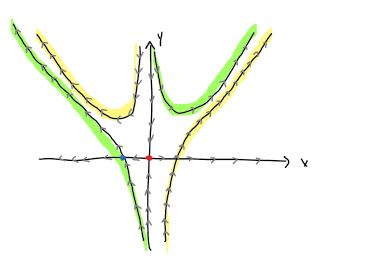
\includegraphics[width=0.8\textwidth]{phasenpotrait.jpeg}
    \end{center}

    Die Informationen über die Richtung der Pfeile erhalten wir daher, dass der Eigenwert in $x$-Richtung $-1$ war, also in Richtung der $x$-Achse die Lösungen von Gleichgewichtspunkt weglaufen. In $y$-Richtung war der Eigenwert $-1$, d.h. Lösungen, die auf der $y$-Achse starten, werden zum Gleichgewichtspunkt hingezogen.
\end{enumerate}


\end{document}